\newpage
\section{Method} \label{sec:method}
\subsection{Setup}
\subsection{Data Set}
The mass spectrometer was set to perform each gas measurement seven times. In this way, seven readings were available for all partial pressures measured at the different mass-to-charge ratios. The values obtained were averaged and the standard deviation of the data was taken as the error. After this was done, only the averaged data were used. 

\subsection{Curve Fit}
\label{sec:fit}
One could add up all the measured partial pressures that belong to the same mass-to-charge ratio. However, this would be less accurate than fitting the measured partial pressures by a {\scshape Gaussian} curve and calculate the area of the curve. 

The peaks were fit to the data with \texttt{scipy.optimize.curve\_fit}\cite{scipy} using a {\scshape Gaussian} peak given in \eqref{eq:gauss}
\begin{align}
    f(x) = A\cdot e^{-\frac{(x-\mu)^2}{2\sigma^2}} \label{eq:gauss}
\end{align}

The fit-function also provides us with the covariance-matrix for the parameters, which allows us to estimate their errors.  
An example is shown in figure \ref{fig:gauss_int}. In order to get the amount of the measured compound we have to calculate the area of the fit. If we just summed up the bins from $\mu-3\sigma$ to $\mu+3\sigma$, but then we also include the noise. The area can directly be calculated from the {\scshape Gaussian} as
\begin{align}
    \int_{-\infty}^{+\infty} A\cdot e^{-\frac{(x-\mu)^2}{2\sigma^2}} \mathrm{d}x = \sqrt{2\pi}A\sigma. \label{eq:gauss_int} 
\end{align}
\begin{figure}[h!]
    \centering
    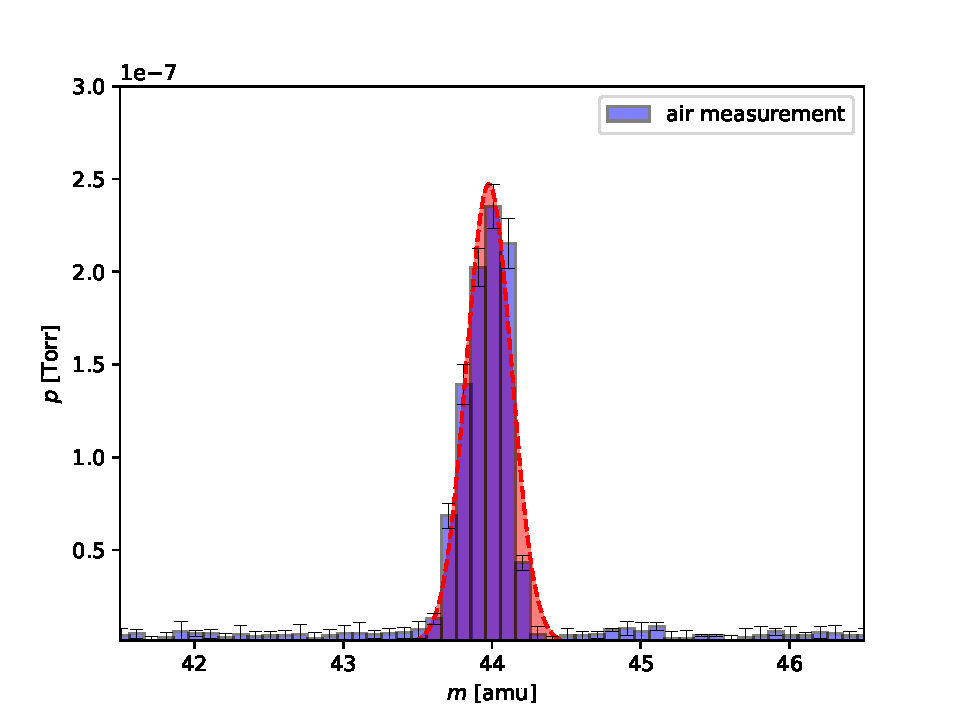
\includegraphics[width=\textwidth]{Report/DataResultsPlots/peak.pdf}
    \caption{An example of our fit applied to a data-set gathered during this experiment.}
    \label{fig:gauss_int}
\end{figure}
For Xenon the peaks at $m=132$ amu/e and $m=131$ amu/e and $m=129$ amue/e overlap, thus a superposition of three {\scshape Gaussians} separated by $\Delta m_1 = 1$ amu/e and $\Delta m_2 = 3$ amu/e was used to fit the peaks, this equation is given in \eqref{eq:gaussxe}.
\begin{align}
    f(x) = A_1\cdot e^{-\frac{(x-\mu)^2}{2\sigma_1^2}} + A_2\cdot e^{-\frac{(x-\mu - 1)^2}{2\sigma_2^2}} + A_3\cdot e^{-\frac{(x-\mu-3)^2}{2\sigma_3^2}} \label{eq:gaussxe}
\end{align}

The mass-to-charge ratio of a double-ionised isotope is half that of a single-ionised isotope and therefore does not have to be an integer. Peaks can lie next to each other at a distance of half an amu/e.  Since the resolution used is not sufficient, the peaks in case of double-ionised xenon isotopes can overlap so much that some peaks cannot be recognised as local maximum in the partial pressure. Therefore, we could not work with the fit-function for such positions. In such cases, we estimated the amplitude of the {\scshape Gaussian} curve as the partial pressure at the position where the peak would be expected. It's error was estimated as the error of the partial pressure.  For the standard deviation we chose $\sigma = 0.2 \pm 0.1$ amu which is except for the generous error about the same as for the other peaks. 

The detection of the peaks was automated. A threshold had to be defined to ensure that detected peaks are not random and that they are distinct enough to make a {\scshape Gaussian} fit. We set the condition that three peaks next to each other must deviate significantly from zero. Furthermore, this had to be at integer or half-integer amu/e values. 
For all other measures no {\scshape Gaussian} curves were produced and the partial pressure at these locations was assumed to be zero.

\subsection{Calibration}
Upon looking at the fit Peaks for Argon and Xenon, we noticed that there was a slight deviation from the expected location. We thus had to calibrate the measurement of the detector with this two data-sets. Equation \eqref{eq:calibrate} was applied to all gathered data in order to calibrate the $m/q$ axis.
\begin{align}
    m \to m_\text{Ag, true} + \frac{m_\text{Xe, true} - m_\text{Ag, true}}{m_\text{Xe, fit} - m_\text{Ag, fit}} \cdot (m - m_\text{Ag, fit}) \label{eq:calibrate}
\end{align}
Where $m_{i, \text{true}}$ are taken from literature and $m_{i, \text{fit}}$ are obtained from our fit.
The error on this calibration is derived in \ref{app:err_cal}.

\subsection{Component identification}

Using the {\scshape Gaussian} fit described in the upper part, it was now possible to simplify the data set so that only one partial pressure is assigned to each integer or half-integer mass-to-charge ratio. 

In order to estimate which gas components make up the partial pressure of individual mass-to-charge ratios, we used data from \texttt{NIST}. These data sets contain at which $m/q$ which partial pressure is to be expected in a measurement with a mass spectrometer. The partial pressures are given relative to each other and normalised in such a way that the mass-to-charge ratio that occurs most is assigned the value one. \texttt{NIST} data of Xe, Ar, Kr, propane, butane, isobutane, ethanol, H$_2$O, CO$_2$, N$_2$, H$_2$O, O$_2$, H$_2$ were considered in this thesis. We wrote an algorithm which checks for each substance $i$ whether the mass-to-charge ratio which is most represented $A_{\mathrm{max}~i}$ is also present in our measurements. If so, the \texttt{NIST} ratios of substance $i$ are scaled so that their value at $A_{\mathrm{max}~i}$ exactly matches the measured partial pressure (see figure \ref{fig:illustration_nist1} substance $i$). If $A_{\mathrm{max~j}}$ of a substance $j$ is already occupied by an other substance, the \texttt{NIST} values of substance $j$ were scaled only to such an extent that, partial pressure of the two gasses at $A_{\mathrm{max}~j}$ added together matches the measured value (see fig \ref{fig:illustration_nist1} substance $j$).  

\begin{figure}[h!]
    \centering
    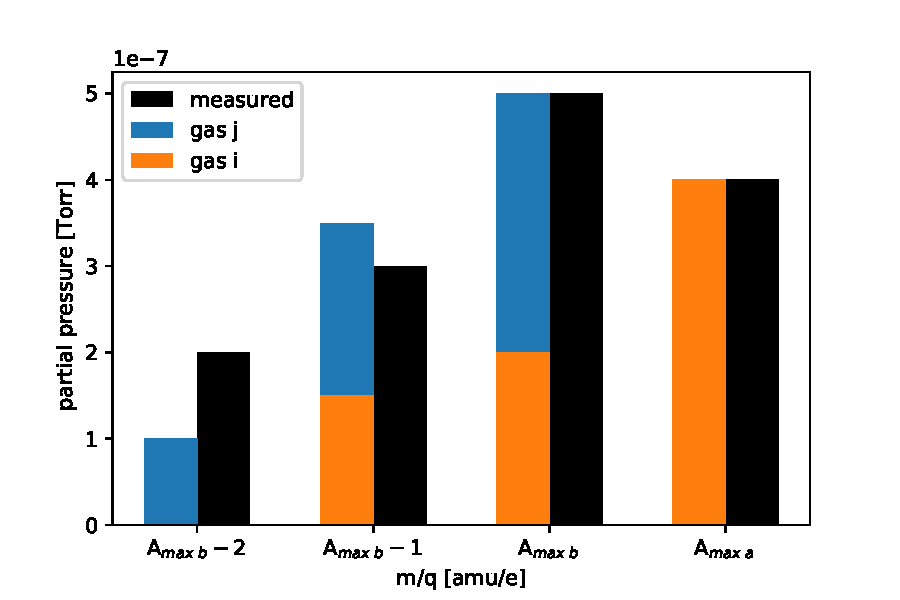
\includegraphics[width=\textwidth]{Report/DataResultsPlots/ilustration_nist_approx1.pdf}
    \caption{Illustration of first kind of \texttt{NIST} approximation}
    \label{fig:illustration_nist1}
\end{figure}

This procedure is only applicable as long as one of the two overlapping substances has its maximum at a mass-to-charge ratio which is not occupied by any other substance.  In the case of propane, butane and isobutane, the maximum of each substance is also represented by the other two substances. To make sure that the approximation at the mass-to-charge ratio where the substances have their maxima correspond exactly to the measured values, we set up the following system of equations  
\begin{align} \label{eq:coef1}
    p_{43} = \alpha_{\mathrm{pro}}\cdot r_\mathrm{pro43} + \alpha_\mathrm{but} \cdot r_\mathrm{but43} + \alpha_\mathrm{iso}\cdot r_\mathrm{iso43} \\
    \label{eq:coef2}
    p_{41} = \alpha_{\mathrm{pro}}\cdot r_\mathrm{pro41} + \alpha_\mathrm{but} \cdot r_\mathrm{but41} + \alpha_\mathrm{iso}\cdot r_\mathrm{iso41} \\
    \label{eq:coef3}
    p_{29} = \alpha_{\mathrm{pro}}\cdot r_\mathrm{pro29} + \alpha_\mathrm{but} \cdot r_\mathrm{but29} + \alpha_\mathrm{iso}\cdot r_\mathrm{iso29},
\end{align}
where $p_k$ is the measured partial pressure and $r_{\mathrm{pro}k}$, $r_{\mathrm{but}k}$ and $r_{\mathrm{iso}k}$ are partial pressure ratios according to the \texttt{NIST} data for propane, butane and isobutane at mass-to-charge ratio $k$. 29 amu/e is the maximum of propane, 43 amu/e is the maximum of butane and 41 amu/e the second highest ratio of isobutane (the highest would also be 43 mass-to-charge ratio). $\alpha_\mathrm{but}$, $\alpha_\mathrm{pro}$ and $\alpha_\mathrm{iso}$ are the unknown coefficients to scale the partial pressure ratios. This equation can be easily solved for the three unknown scale factors. 

In this way, a gas composition was automatically calculated that would roughly explain our measured values. This allows us to assess whether our measurements are meaningful. Therefore, these \texttt{NIST} approximations were often plotted next to the measured values. In the following, this type of component estimation is called first kind of \texttt{NIST} approximation. 

\subsection{Component estimation}

In many cases the first kind of \texttt{NIST} approximations differ strongly from the measured partial pressures (illustrated in figure \ref{fig:illustration_nist1} in the left two bars). Since we want to work with our measured values and not with the approximations to determine the gas ratios, we scaled the approximations for each m/q so that their bar height matches that of the measured data (see figure \ref{fig:illustration_nist2}). In this way, measured partial pressures that can only be caused by one type of substance are completely assigned to that type. However, if partial pressures can be explained by more than one type of molecule, they are assigned to the respective substance in the same proportion as the approximation is divided. This second kind of \texttt{NIST} approximation is used to estimate the ratio of the gas components but it can't be used to assess how accurate our measurements can be explained by a gas mix. 

\begin{figure}[h!]
    \centering
    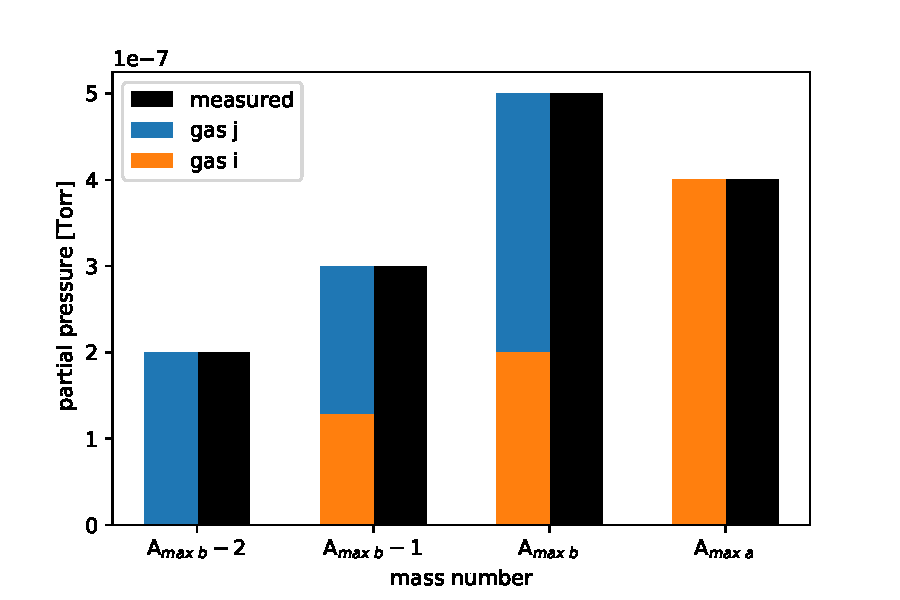
\includegraphics[width=\textwidth]{Report/DataResultsPlots/ilustration_nist_approx2.pdf}
    \caption{Illustration of the second kind of approximation by \texttt{NIST} data. }
    \label{fig:illustration_nist2}
\end{figure}

After the procedure for determining the gas ratios and building the two approximations has been described qualitatively, it is written down mathematically in the following section for the sake of completeness. 
The partial pressure of a substance $m$ is calculated as
\begin{align}
   p_m = \sum_{k~in~A} {p_{m_k}}, 
\end{align}
where $p_{m_k}$ is the partial pressure of this substance with mass-to-charge ratio $k$ according to the second kind of approximation and $A$ are all the mass-to-charge ratios which occur with this substance. 


The partial pressure $p_{m_k}$ can be calculated as 
\begin{align}
    p_k\cdot \kappa_{m_k}.
\end{align}
 Here $p_k$ is the measured partial pressure at mass-to-charge ratio $k$ and $\kappa_{m_k}$ is the ratio of the partial pressure due to substance $m$ at this location. The ratio $\kappa_{m_k}$ is determined as 
 \begin{align}
     \kappa_{m_k} = \frac{p_{m_k}'}{p_{k}'}.
 \end{align}
 
In this equation $p_{k}'$ is the partial pressure and $p_{m_k}'$ is the partial pressure due to substance $m$ according to the first kind of approximation. The first kind of approximation was done by calculating the scale factor $\alpha_m$ for each substance. Here $\alpha_m$ is the factor, the \texttt{NIST} ratios $r_{m_k}$ of the substance must be multiplied with to obtain $p_{m_k}$. The scale factor $\alpha_m$ is equal to the measured partial pressure at $A_{{max}~m}$ minus the partial pressure already occupied by other substances or in the case of propane, butane and isobutane the coefficients are calculated according to (\ref{eq:coef1}), (\ref{eq:coef2}) and (\ref{eq:coef3}). The error estimation of this part can be seen in the appendix. 






